\documentclass[reqno,12pt,letterpaper]{amsart}
\RequirePackage{amsmath,amssymb,amsthm,graphicx,mathrsfs,url,slashed}
\RequirePackage[usenames,dvipsnames]{xcolor}
\RequirePackage[colorlinks=true,linkcolor=Red,citecolor=Green]{hyperref}
\RequirePackage{amsxtra}
\usepackage{cancel}
\usepackage{tikz-cd}

\setlength{\textheight}{9.3in} \setlength{\oddsidemargin}{-0.25in}
\setlength{\evensidemargin}{-0.25in} \setlength{\textwidth}{7in}
\setlength{\topmargin}{-0.25in} \setlength{\headheight}{0.18in}
\setlength{\marginparwidth}{1.0in}
\setlength{\abovedisplayskip}{0.2in}
\setlength{\belowdisplayskip}{0.2in}
\setlength{\parskip}{0.05in}
\renewcommand{\baselinestretch}{1.05}

\title[Hyperbolic least-gradient maximum principle]{The least-gradient maximum principle on hyperbolic manifolds}
\author{Aidan Backus}
\date{May 2022}

\newcommand{\NN}{\mathbf{N}}
\newcommand{\ZZ}{\mathbf{Z}}
\newcommand{\QQ}{\mathbf{Q}}
\newcommand{\RR}{\mathbf{R}}
\newcommand{\CC}{\mathbf{C}}
\newcommand{\DD}{\mathbf{D}}
\newcommand{\PP}{\mathbf P}
\newcommand{\MM}{\mathbf M}
\newcommand{\II}{\mathbf I}
\newcommand{\Hyp}{\mathbf H}
\newcommand{\Sph}{\mathbf S}
\newcommand{\GL}{\mathbf{GL}}
\newcommand{\Orth}{\mathbf{O}}
\newcommand{\Ball}{\mathbf{B}}

\DeclareMathOperator{\card}{card}
\DeclareMathOperator{\cent}{center}
\DeclareMathOperator{\ch}{ch}
\DeclareMathOperator{\codim}{codim}
\DeclareMathOperator{\diag}{diag}
\DeclareMathOperator{\diam}{diam}
\DeclareMathOperator{\dom}{dom}
\DeclareMathOperator{\Exc}{Exc}
\DeclareMathOperator{\Gal}{Gal}
\DeclareMathOperator{\Hom}{Hom}
\DeclareMathOperator{\Iso}{Iso}
\DeclareMathOperator{\Jac}{Jac}
\DeclareMathOperator{\Lip}{Lip}
\DeclareMathOperator{\Met}{Met}
\DeclareMathOperator{\id}{id}
\DeclareMathOperator{\rad}{rad}
\DeclareMathOperator{\rank}{rank}
\DeclareMathOperator{\Hess}{Hess}
\DeclareMathOperator{\Radon}{Radon}
\DeclareMathOperator*{\Res}{Res}
\DeclareMathOperator{\sgn}{sgn}
\DeclareMathOperator{\singsupp}{sing~supp}
\DeclareMathOperator{\Spec}{Spec}
\DeclareMathOperator{\supp}{supp}
\DeclareMathOperator{\Tan}{Tan}
\newcommand{\tr}{\operatorname{tr}}

\newcommand{\Ric}{\mathrm{Ric}}
\newcommand{\Riem}{\mathrm{Riem}}
\newcommand*\dif{\mathop{}\!\mathrm{d}}
\newcommand{\LapQL}{\Delta^{\mathrm{ql}}}

\newcommand{\dbar}{\overline \partial}

\DeclareMathOperator{\atanh}{atanh}
\DeclareMathOperator{\csch}{csch}
\DeclareMathOperator{\sech}{sech}

\DeclareMathOperator{\Div}{div}
\DeclareMathOperator{\Gram}{Gram}
\DeclareMathOperator{\grad}{grad}
\DeclareMathOperator{\dist}{dist}
\DeclareMathOperator{\spn}{span}
\DeclareMathOperator{\Ell}{Ell}
\DeclareMathOperator{\WF}{WF}

\newcommand{\Lagrange}{\mathscr L}
\newcommand{\DirQL}{\mathscr D^{\mathrm{ql}}}
\newcommand{\DirL}{\mathscr D}

\newcommand{\Hilb}{\mathcal H}
\newcommand{\Homology}{\mathrm H}
\newcommand{\normal}{\mathbf n}
\newcommand{\radial}{\mathbf r}
\newcommand{\evect}{\mathbf e}
\newcommand{\vol}{\mathrm{vol}}

\newcommand{\pic}{\vspace{30mm}}
\newcommand{\dfn}[1]{\emph{#1}\index{#1}}

\renewcommand{\Re}{\operatorname{Re}}
\renewcommand{\Im}{\operatorname{Im}}

\newcommand{\loc}{\mathrm{loc}}
\newcommand{\cpt}{\mathrm{cpt}}

\def\Japan#1{\left \langle #1 \right \rangle}

\newtheorem{theorem}{Theorem}[section]
\newtheorem{badtheorem}[theorem]{``Theorem"}
\newtheorem{prop}[theorem]{Proposition}
\newtheorem{lemma}[theorem]{Lemma}
\newtheorem{sublemma}[theorem]{Sublemma}
\newtheorem{claim}[theorem]{Claim}
\newtheorem{proposition}[theorem]{Proposition}
\newtheorem{corollary}[theorem]{Corollary}
\newtheorem{conjecture}[theorem]{Conjecture}
\newtheorem{axiom}[theorem]{Axiom}
\newtheorem{assumption}[theorem]{Assumption}

\theoremstyle{definition}
\newtheorem{definition}[theorem]{Definition}
\newtheorem{remark}[theorem]{Remark}
\newtheorem{example}[theorem]{Example}
\newtheorem{notation}[theorem]{Notation}

\newtheorem{exercise}[theorem]{Discussion topic}
\newtheorem{homework}[theorem]{Homework}
\newtheorem{problem}[theorem]{Problem}

\newtheorem{ack}{Acknowledgements}

\numberwithin{equation}{section}


% Mean
\def\Xint#1{\mathchoice
{\XXint\displaystyle\textstyle{#1}}%
{\XXint\textstyle\scriptstyle{#1}}%
{\XXint\scriptstyle\scriptscriptstyle{#1}}%
{\XXint\scriptscriptstyle\scriptscriptstyle{#1}}%
\!\int}
\def\XXint#1#2#3{{\setbox0=\hbox{$#1{#2#3}{\int}$ }
\vcenter{\hbox{$#2#3$ }}\kern-.6\wd0}}
\def\ddashint{\Xint=}
\def\dashint{\Xint-}

\usepackage[backend=bibtex,style=alphabetic]{biblatex}
\renewcommand*{\bibfont}{\normalfont\footnotesize}
\addbibresource{topics.bib}
\renewbibmacro{in:}{}
\DeclareFieldFormat{pages}{#1}


\begin{document}
\begin{abstract}
The least-gradient maximum principle, essentially due to Miranda and de Giorgi in the 1960s, shows that least-gradient functions define a minimal lamination of the support of their derivative.
We show that this result still holds on hyperbolic manifolds.
As a consequence we answer some questions of Daskalopoulos--Uhlenbeck concerning the $L^\infty$-Teichm\"uller theory.
\end{abstract}

\maketitle

%%%%%%%%%%%%%%%%%%%%%%%%%%%%%%%%%%%%%%%%%%%%%%%%%%%%%%%

% \tableofcontents

\section{Introduction}
Throughout this paper, let $M$ be an oriented Riemannian manifold of metric $g$ and dimension $d$.
For a function $u \in BV_\loc(M)$, we write $\star |\dif u|$ for the total variation of the derivative, c.f. (\ref{total variation}).

\begin{definition}\label{main definitions}
A function $u \in BV_\loc(M)$ has \dfn{least gradient} if for every $v \in BV_\cpt(M)$ such that $\supp v \subseteq U \Subset M$,
$$\int_U \star |\dif u| \leq \int_U \star |\dif u + \dif v|.$$
A set $U$ of locally finite perimeter has \dfn{least perimeter} if $1_U$ has least gradient.
\end{definition}

Functions of least gradient arise naturally in conductivity imaging \cite{Nachman2009, Tamasan2019} as well as the formal limit of $p$-harmonic functions as $p \to 1$, but we are interested in them primarily because of their applications to minimal surfaces and the $L^\infty$-Teichm\"uller theory of Thurston and Daskalopoulos--Uhlenbeck \cite{thurston1998minimal,daskalopoulos2020transverse}.
In that context one is interested in the existence of minimal laminations in a closed hyperbolic manifold, as defined below:

\begin{definition}
A \dfn{minimal lamination} in $M$ is a partition of a closed subset of $M$ into smooth hypersurfaces with zero mean curvature.
The minimal lamination $\lambda$ is \dfn{analytic} if $(M, g)$ is analytic and each of the hypersurfaces in $\lambda$ is analytic.
\end{definition}

Our first theorem is an analogue of the maximum principle for least gradient functions on euclidean space \cite[Proposition 3.4]{górny2017planar}.

\begin{theorem}[maximum principle]\label{main thm}
Suppose that $2 \leq d \leq 7$ and suppose that $M$ has negative constant curvature.
Let $u: M \to \RR$ be a function of least gradient, and $A_y = \partial \{u > y\}$.
Then $(A_y)_{y \in \RR}$ is an analytic minimal lamination in $M$, and each $A_y$ is a locally finite union of connected minimal hypersurfaces.
\end{theorem}

Theorem \ref{main thm} partially answers a question \cite[Problem 9.5]{daskalopoulos2020transverse} of Daskalopoulos--Uhlenbeck; we state this as Corollary \ref{maximum stretch contains lamination}.
Moreover, in the course of proving Theorem \ref{main thm}, we shall obtain as a byproduct a solution to \cite[Problem 9.7]{daskalopoulos2020transverse}, namely Corollary \ref{ruelle sullivan antiderivative}.

Theorem \ref{main thm} is a consequence of the following regularity theorem for sets of least perimeter.

\begin{theorem}[regularity of minimal hypersurfaces]\label{main lma}
Suppose that $2 \leq d \leq 7$.
Then every set of least perimeter in $\Hyp^d$ is bounded by an analytic minimal hypersurface $N$.
\end{theorem}

Analogous results to Theorem \ref{main lma} include regularity of minimal currents weighted by an elliptic integrand, proven by Federer \cite[\S5.3]{federer2014geometric}, and regularity of sets of least perimeter on $\RR^d$ developed by Miranda \cite{Miranda64, Miranda66, Miranda67}.
Our strategy closely mirrors Miranda's, and in this paper we emphasize the steps of the proof where significant modifications of Miranda's arguments are necessary.

\begin{proof}[Proof of Theorem \ref{main thm}]
We first pass to the universal cover of $M$, which is an open subset of $\Hyp^d$.
By Proposition \ref{level sets are minimal}, for every function $u$ of least gradient, the superlevel sets of $u$ have least perimeter.
Let
\begin{equation}\label{lamination union}
A = \bigcup_y \partial \{u > y\},
\end{equation}
let $B$ be the interior of $\{du = 0\}$, and let $x \in M$.
Then $x \in B$ iff $u = u(x)$ near $x$, but that happens iff for every $y < u(x)$, $x$ is interior to $\{u > y\}$ and for every $y \geq u(x)$, $x$ is exterior to $\{u > y\}$.
This happens iff for every $y \in \RR$, $x$ is either interior or exterior to $\{u > y\}$, thus $x \notin \partial \{u > y\}$, which happens iff $x \notin A$.
Thus $\{A, B\}$ is a partition of $M$, so $A$ is closed.
Moreover, the sets $\{u > y\}$ are totally ordered by $\subseteq$, so the sets $\partial \{u > y\}$ are disjoint.
They are also hypersurfaces with the desired amount of regularity, by Theorem \ref{main lma}.
By Proposition \ref{local finiteness} the decomposition of $\partial \{u > y\}$ into connected components is locally finite.
\end{proof}

It was shown by G\'orny that functions of least gradient on $\RR^d$, $d \leq 7$, have a decomposition into continuous and jump parts \cite[Theorem 1.2]{górny2017planar}.
We assert that given Theorem \ref{main thm}, the proof of this result goes through verbatim:

\begin{theorem}[G\'orny's regularity theorem]\label{Gorny regularity}
Let $M$ be an open bounded strictly convex manifold of constant negative curvature and dimension $\leq 7$.
Then any function of least gradient $u: M \to \RR$ can be written as the sum of a continuous function of least gradient, and a function of least gradient with only jump discontinuities.
\end{theorem}

TODO: Check this very carefully

%%%%%%%%%%%%%%%%%%%%%%%%%%%%%%%%%%%%%%%%%%%%%%%

\subsection{Applications to hyperbolic geometry}
In this section we discuss applications to Teichm\"uller theory and hyperbolic computational geometry.

The Thurston asymmetric metric, first defined in \cite{thurston1998minimal}, is constructed from best-Lipschitz maps between two closed hyperbolic manifolds.
As a first step towards an analytic understanding of the Thurston asymmetric metric, Daskalopoulos--Uhlenbeck \cite{daskalopoulos2020transverse} considered best-Lipschitz maps $M \to S^1$ where $M$ is a closed hyperbolic surface.
They identified a particularly important class of such maps, the $\infty$-harmonic maps, defined as follows, which are particularly significant because they induce geodesic laminations of $M$.

\begin{definition}
If a function $u$ is the weak limit in $L^r$ for $r > d$ of $p$-harmonic functions as $p \to \infty$, we call $u$ \dfn{$\infty$-harmonic}.
For an $\infty$-harmonic function $u$ we define the \dfn{maximum-stretch locus}
$$\lambda_u := \{x \in M: L(x) = \sup L\}$$
where $L(x)$ denotes the local Lipschitz constant of $u$ at $x$.
\end{definition}

\begin{theorem}\label{infinity harmonic laminations}
Suppose that $M$ is a closed hyperbolic surface and $u$ is an $\infty$-harmonic function. Then the maximum-stretch locus $\lambda_u$ is a geodesic lamination in $M$.
\end{theorem}

In \cite[\S5]{daskalopoulos2020transverse}, Daskalopoulos--Uhlenbeck prove the above theorem by considering the viscosity solution theory of $\infty$-Laplace equation
\begin{equation}\label{infinity laplace}
    \Hess u(\grad u, \grad u) = 0.
\end{equation}
However, the theory of viscosity solutions of (\ref{infinity laplace}) is still nascent, and Daskalopoulos--Uhlenbeck ask for a proof of Theorem \ref{infinity harmonic laminations} that bypasses (\ref{infinity laplace}) altogether, c.f. \cite[Problem 9.5]{daskalopoulos2020transverse}.
We give a partial resolution of this problem by proving \cite[Theorem-Conjecture 9.6]{daskalopoulos2020transverse}.
Before stating it we note that by a \dfn{section of least gradient} $u$ we mean a section that lifts to a section $\tilde u$ on $\Hyp^d$, such that $\tilde u$ can be trivialized to a function of least gradient

\begin{corollary}\label{maximum stretch contains lamination}
Let $u$ be an $\infty$-harmonic function on a closed hyperbolic surface $M$.
Then the maximum-stretch locus $\lambda_u$ contains a geodesic lamination.
\end{corollary}
\begin{proof}
By \cite[\S6]{daskalopoulos2020transverse}\footnote{The proof that such a section exists does not use Theorem \ref{infinity harmonic laminations}.}, there exists an affine bundle $E \to M$ and a section $v$ of least gradient of $E$ such that $\supp \dif v \subseteq \lambda_u$.
By Theorem \ref{main thm}, $\supp \dif v$ is a geodesic lamination.
\end{proof}

It is not clear that $\supp \dif v = \lambda_u$ in the above corollary, essentially because it is not clear that the map $\dif u \mapsto \dif v$ is locally injective (so $\dif v$ could be $0$ somewhere on $\lambda_u$).
We believe that this should be true, and state this as Conjecture \ref{two laminations agree}.

Daskalopoulos--Uhlenbeck also ask for a partial converse to the fact that $\dif v$ endows $\lambda_u$ with the structure of an oriented measured lamination.
We now prove this, resolving \cite[Problem 9.7]{daskalopoulos2020transverse}.
For the definition of the Ruelle-Sullivan $1$-current of an oriented, transversely measured geodesic lamination, see \cite[\S8]{daskalopoulos2020transverse} or the original paper of Ruelle--Sullivan \cite{Ruelle75}.

\begin{proposition}\label{minimal bounding implies least gradient}
Let $u \in BV_\loc(M)$, where $M$ is a hyperbolic manifold, and suppose that the level sets $\partial \{u > y\}$ define a minimal lamination.
Then $u$ is a function of least gradient.
\end{proposition}
\begin{proof}
Fix $U \Subset M$ and let $v$ be a competitor in $U$, thus $v \in BV(U)$ and $u - v$ is trace-free.
Then for $T: BV(U) \to L^1(U)$ the trace map, $\{Tu > y\} = \{Tv > y\}$ by (\ref{convergence of trace}).
It follows that $\partial^* \{v > y\}$ is a competitor to $\partial \{u > y\}$ in $U$ and hence, since $\partial \{u > y\}$ is minimal,
$$|\partial^* \{u > y\} \cap U| \leq |\partial^* \{v > y\} \cap U|.$$
That $u$ has least gradient now follows from the coarea formula, Proposition \ref{coarea formula}.
\end{proof}

\begin{corollary}\label{ruelle sullivan antiderivative}
Let $\lambda$ be an oriented, transversely measured geodesic lamination on a closed hyperbolic surface $M$, and let $\dif v$ be the Ruelle-Sullivan $1$-current induced by $\lambda$.
Then $\dif v$ is the derivative of a section of least gradient $v: M \to E$, for some affine bundle $E \to M$.
\end{corollary}
\begin{proof}
As observed in \cite[\S9]{daskalopoulos2020transverse}, if we lift $\dif v$ to a $1$-current $\dif \tilde v$ on $\Hyp^2$, then $\dif \tilde v$ is exact and any antiderivative $\tilde v$ of $\dif \tilde v$ has superlevel sets $\{\tilde v \geq y\}$ which are bounded by geodesics.
Moreover we can choose $\tilde v$ to be $\pi_1(M)$-equivariant.
The claim now follows from Proposition \ref{minimal bounding implies least gradient} and the realization of $\pi_1(M)$-equivariant functions on $\Hyp^2$ as sections of an affine bundle, c.f. \cite[\S4]{daskalopoulos2020transverse}.
\end{proof}

When combined with work of Loisel \cite{Loisel20}, Theorem \ref{main thm} also finds application in computational hyperbolic geometry, as it furnishes a large class of minimal laminations which are inexpensive to compute.

\begin{proposition}\label{cohomology makes laminations}
Let $M$ be a closed hyperbolic manifold of dimension $d \leq 7$, and let $\alpha \in H^1(M, \RR)$.
Then there is a natural minimal lamination $\lambda$ in $M$ induced by $\alpha$, which can be obtained by solving a least-gradient Dirichlet problem on a fundamental polytope of $M$.
\end{proposition}
\begin{proof}
Let $\Gamma = \pi_1(M)$. The Hurcewiz theorem implies that $\alpha$ pulls back to a map $\Gamma \to \RR$.
Then $\alpha$ is a representation of $\Gamma$ and thus induces a space $E$ of equivariant functions on the boundary $\Omega$ of each fundamental polytope $\Omega$ of $\Gamma$. To be more precise, for every $f \in E$ and $\gamma \in \Gamma$,
\begin{equation}\label{boundary data for Loisel}
f(\gamma x) = f(x) + \alpha(\gamma),
\end{equation}
and $f$ is constant on each face of $\partial \Omega$.
The relation (\ref{boundary data for Loisel}) is an underdetermined boundary condition for functions in $E$, and so we consider the subspace $E'$ of functions which in addition are zero on a maximal set of faces such that we do not determine $f|\partial \Omega = 0$, thus any function $E' \subseteq E$ has a completely determined trace $t$ on $\partial \Omega$.
It follows from \cite[Theorem 4.4]{daskalopoulos2020transverse} that there exists a function $u$ of least gradient on $\Omega$ whose trace is $t$.
The minimal lamination induced by a function $u \in E$ of least gradient from Theorem \ref{main thm} does not depend on the class of $u$ in $E/E'$, since that is a space of constants; so we obtain a uniquely defined minimal lamination of $M$.
\end{proof}

\begin{corollary}
With $M, \alpha, \lambda$ as in Proposition \ref{cohomology makes laminations}, and every quasiuniform triangulation $T$ of $M$, there exists a numerical algorithm for computing $\lambda$ with finite elements in $T$ with time complexity $O(|T|^{1/2} \log |T|)$ where $|\cdot|$ is cardinality.
\end{corollary}
\begin{proof}
By \cite[Theorem 1]{Loisel20}, one can solve the least-gradient Dirichlet problem with finite elements in $T$ with time complexity $O(|T|^{1/2} \log |T|)$.
\end{proof}

TODO: Do some numerical experiments, show what minimal laminations in a fundamental polytope in $\Hyp^3$ look like


%%%%%%%%%%%%%%%%%%%%%%%%%%%%%%%%%%%%%%%%%%%%%%%

\subsection{Some open problems}
We believe that Theorem \ref{main lma} could be extended to a wider class of Riemannian manifolds:

\begin{conjecture}\label{main conj}
Suppose that $2 \leq d \leq 7$ and $M$ is a simply connected Riemannian $d$-fold. Then Theorem \ref{main lma} holds with $\Hyp^d$ replaced by $M$.
\end{conjecture}

This conjecture implies Theorem \ref{main thm} for arbitrary $M$ by passing to the universal cover.
Since our proof strongly uses the symmetries of $\Hyp^d$, it would be reasonable to first try to prove Conjecture \ref{main conj} for locally homogeneous manifolds, and especially those locally homogeneous manifolds $M$ such that for every $P \in M$ there is a natural action of $\Orth(\RR^d)$ on $M$ by isometry that fixes $P$.
Another line of attack would be to show that our methods are perturbative, so that if $(M, g)$ is a simply connected Riemannian manifold such that $g$ is ``close to constant negative curvature'' in some sense, then Conjecture \ref{main conj} holds for $(M, g)$.

It seems highly unlikely that Theorem \ref{main lma} can be extended to $\Hyp^8$, due to the existence of Simons cones in $\RR^8$ \cite[Theorem A]{BOMBIERI1969}.
Simons cones are not of least perimeter in $\Hyp^8$, but one could potentially perturb them to obtain a set of least perimeter whose boundary is singular:

\begin{problem}
    Construct a set $U$ of least perimeter in $\Hyp^8$ such that $\partial U$ has a singularity of codimension $8$.
\end{problem}

Owing to the G\'orny regularity theorem, Theorem \ref{Gorny regularity}, we suspect that its consequence \cite[Theorem 1.1]{górny2017planar} holds, giving well-posedness for the Dirichlet problem in strictly convex planar domains.
However, this is not obvious as we have not extended the Sternberg--Williams--Ziemer theorem \cite{ZiemerWilliamsSternberg1992} to the hyperbolic case.
We therefore state G\'orny's main theorem as a conjecture:

\begin{conjecture}
Let $U$ be an open, bounded, strictly convex subset of $\Hyp^2$ with $C^1$ boundary.
Then there exists a solution of the least-gradient Dirichlet problem on $U$ with data in $BV(\partial U)$.
\end{conjecture}

We would also like to know that the $\infty$-harmonic/least-gradient duality gives a complete proof of Theorem \ref{infinity harmonic laminations}, which follows from the below conjecture.

\begin{conjecture}\label{two laminations agree}
Let $u$ be an $\infty$-harmonic function with dual least-gradient section $v$.
Then $\supp \dif v = \lambda_u$.
\end{conjecture}

%%%%%%%%%%%%%%%%%%%%%%%%%%%%%%%%%%%%%%%%%%%%%%%

\subsection{Outline of the paper}
We begin with the preliminaries in \S\ref{LeastGradientFunctions} by developing the theory of functions of least gradient on Riemannian manifolds. A generalization of Miranda's theorem \cite[Teorema 3]{Miranda67} on the stability of functions of least gradient, and generalizations of its standard consequences, easily fall out.
In particular, we show that the tangent cone to a set of least perimeter exists and is a hyperplane.
We also prove a monotonicity formula and its consequences.

We are then ready to prove Theorem \ref{main lma}.
In \S\ref{MollifierSection}, we show Proposition \ref{mollifier quant}, which says that a set of least perimeter can be approximated by $C^1$ hypersurfaces that are approximately minimal.
This result is then used in \S\ref{DeGiorgiSection} to prove Theorem \ref{main lma}. We do this by proving an analogue of the de Giorgi regularity lemma \cite[Teorema 5.7]{Miranda66} for $\Hyp^d$. The de Giorgi lemma is the only point of the proof where we use the constant negative curvature of $M$.
We rely on the transitivity of $\Iso(\Hyp^d)$ as well as the fact that one can represent hypersurfaces in $\Hyp^d$ on euclidean space in a way which approximately preserves the surface area and normal vector field.

%%%%%%%%%%%%%%%%%%%%%%%%%%%%%%%%%%%%%%%%%%%%%%%%

\subsection{Acknowledgements}
I would like to thank Georgios Daskalopoulos for suggesting this project and for many helpful discussions.
I would also like to thank Joshua Lin for suggesting the proof of Lemma \ref{cross product formula}.

\section{Functions of least gradient}\label{LeastGradientFunctions}
\subsection{Riemannian measure theory}
Let us recall some measure-theoretic facts.
See \cite[Chapter 1]{Giusti77} for analogous results over $\RR^d$, and see \cite{simon1983GMT} for the definition of a de Rham current.
We write $\int_U \omega \wedge \psi$ for the pairing of an $\ell$-current $\omega$ with a compactly supported $\ell$-form $\psi$ in an open set $U$.
We identify the distributional derivative of a function $u$ with the $d-1$-current
$$\int_U \dif u \wedge \psi = -\int_U u \wedge \dif \psi.$$
A function $u$ is in $BV(U)$ iff its derivative $\dif u$ has finite total variation
\begin{equation}\label{total variation}
\int_U \star |\dif u| := \sup_{\substack{||\psi||_{L^\infty} \leq 1\\\supp \psi \Subset V}} \int_U \dif u \wedge \psi.
\end{equation}
Whether a current has locally finite total variation is independent of the Riemannian metric and so $BV_\loc(M)$ is also independently defined.

Now let $u \in BV_\loc(M)$.
Then by \cite[Theorem 4.14]{simon1983GMT}, there exists a $\star |\dif u|$-measurable section $f$ of the cosphere bundle $S'M$ such that for every compactly supported $d-1$-form $\psi$,
\begin{equation}\label{RNy formula}
\int_M \dif u \wedge \psi = \int_M f|\dif u| \wedge \psi.
\end{equation}

For a vector field $X$, we write $\star (Xu) := \dif u \wedge \star (X^\flat)$.
The section $f$ of (\ref{RNy formula}) is given pointwise $\star |\dif u|$-almost everywhere, in any local coordinates $(y_1, \dots, y_d)$, by
\begin{equation}\label{Lebesgue point definition}
    f(x) = \sum_{i = 1}^d \left[\lim_{r \to 0} \frac{\int_{B(x, r)} \star \partial_{y_i} u}{\int_{B(x, r)} \star |\dif u|}\right] ~\dif y^i,
\end{equation}
according to the Besicovitch differentiation theorem; here we view $(\dif y^i)$ as a basis of $T'_xM$.
Whether the limit $f(x)$ in (\ref{Lebesgue point definition}) exists, or indeed its value as a point of $S'_xM$, do not depend on the Riemannian metric or the choice of coordinates.

\begin{definition}
The points $x$ for which the limit (\ref{Lebesgue point definition}) exists and satisfies $|f(x)| = 1$ are called the \dfn{Lebesgue points} of $\dif u$.
\end{definition}

The Lebesgue points are particularly important when $U$ is an indicator function:

\begin{definition}
Let $U$ be a set of locally finite perimeter, and let $u = 1_U$. Then:
\begin{enumerate}
\item The \dfn{measure-theoretic boundary} $\partial U$ is the set of points whose Lebesgue density with respect to $M$ is $\in (0, 1)$.
\item The set of Lebesgue points of $\dif u$ is the \dfn{reduced boundary} $\partial^* U$.
\item The $*|\dif u|$-measurable $1$-form $f$ defined by (\ref{Lebesgue point definition}) is the \dfn{conormal $1$-form} $\normal_U$ to $\partial U$.
\end{enumerate}
\end{definition}

Our definition of reduced boundary and conormal $1$-form follows \cite[Definition 3.3]{Giusti77} and is due to \cite{deGiorgi55}.
See \cite{Battista_2021} for an equivalent definition of reduced boundary on Riemannian manifolds, and see \cite[Chapter 6]{Pugh02} for the definition of Lebesgue density.

\begin{proposition}\label{locality of Caccioppoli}
    Let $U$ be a set of locally finite perimeter with conormal $1$-form $\normal$.
    Then:
    \begin{enumerate}
    \item $\partial^* U$ is either empty or $d-1$-dimensional in the Hausdorff sense, and is $d-1$-rectifiable.
    \item $\partial^* U$ is a dense subset of $\partial U$.
    \item If $\normal$ extends to a continuous $1$-form on $\partial U$, then $\partial^* U = \partial U$ is a $C^1$ hypersurface.
    \item If $\partial^* U = \partial U$ is a smooth hypersurface, then $\normal$ is the conormal $1$-form on $\partial U$ as defined in differential topology, and $\star |\dif 1_U|$ is the induced volume form on $\partial U$.
\end{enumerate}
\end{proposition}
\begin{proof}
Most of the assertions of this proposition are diffeomorphism-invariant, so we may assume that $M = \RR^d$ and appeal to \cite[Chapters 2-4]{Giusti77}.
The proof that $\star |\dif 1_U|$ is the induced volume form is identical to \cite[Example 1.4]{Giusti77}.
\end{proof}

\begin{definition}
Let $M$ be a Riemannian manifold, let $U$ be a set of locally finite perimeter, and let $E$ be a Borel set.
The \dfn{perimeter} of $U$ in $E$ is
$$|E \cap \partial^* U| := \int_E \star |\dif 1_U|.$$
\end{definition}

\begin{proposition}[coarea formula]\label{Coarea2}
Let $M$ be a Riemannian manifold and $u \in BV_\loc(M)$. Then for every open set $E$,
\begin{equation}\label{coarea formula}
\int_E \star |\dif u| = \int_{-\infty}^\infty |E \cap \partial \{u > y\}| \dif y.
\end{equation}
\end{proposition}
\begin{proof}
We follow \cite[Theorem 1.23]{Giusti77}, which first proves (\ref{coarea formula}) for $u \in C^\infty(\RR^d)$ using piecewise linear functions.
Such functions are not available for our purposes; instead we note that if $u \in C^\infty(\RR^d)$ and $u$ has no critical points then (\ref{coarea formula}) follows from Fubini's theorem, the fact that $|E \cap \partial \{u > y\}|$ is the surface area of $E \cap \{u = y\}$ (by Proposition \ref{locality of Caccioppoli}), and the change-of-variables formula.
However the left-hand side of (\ref{coarea formula}) is unaffected by critical points of $u$, and the right-hand side of (\ref{coarea formula}) is unaffected by critical values of $u$ by Sard's theorem.
So (\ref{coarea formula}) holds for $u \in C^\infty(\RR^d)$.

The rest of the proof is identical to \cite[Theorem 1.23]{Giusti77}, so we omit the details.
Taking a sequence in $C^\infty(M)$ that converges to $u$ in $L^1_\loc(M)$\footnote{Recall that $C^\infty(M)$ is not dense in $BV_\loc(M)$.}, and applying Fatou's lemma and the semicontinuity of total variation, we conclude the $\geq$ direction of (\ref{coarea formula}).
Moreover, Stokes' theorem gives that for every $d-1$-form $\psi$ such that $||\psi||_{L^\infty} \leq 1$ and $\supp \psi \Subset E$,
$$\int_E u \wedge \dif \psi = \int_{-\infty}^\infty \int_E |\psi| \star |\dif 1_{\partial \{u > y\}}| \dif y \leq \int_{-\infty}^\infty |E \cap \partial \{u > y\}| \dif y.$$
Taking the supremum over $\psi$ we obtain the direction $\leq$ in (\ref{coarea formula}).
\end{proof}

%%%%%%%%%%%%%%%%%%%%

\subsection{Miranda's theorems}
We now assert Miranda's trace theorem for $BV$ functions and stability theorem for least-gradient functions.
We also recall some a priori estimates for least-gradient functions.

\begin{proposition}[Miranda trace theorem]\label{traces}
Let $U \Subset M$ be an open set with Lipschitz boundary.
For every $u \in BV_\loc(U)$ there exists $v \in L^1_\loc(\partial U)$ such that for every $d-1$-form $\psi$,
\begin{equation}\label{Miranda IBP}
\int_U \dif u \wedge \psi + \int_U u \wedge \dif \psi = \int_{\partial U} v\psi.
\end{equation}
Moreover, for almost every $x \in \partial U$,
\begin{equation}\label{convergence of trace}
\int_{U \cap B(x, \varepsilon)} \star |v(x) - u| \ll \varepsilon^d.
\end{equation}
\end{proposition}
\begin{proof}
The assertion (\ref{Miranda IBP}) is diffeomorphism-invariant and so follows from \cite[Teorema 1]{Miranda67}, and (\ref{convergence of trace}) also follows from that result if we are willing to drop a constant factor.
\end{proof}

To state our a priori estimates we define
$$\eta(u, U) := \inf_{v \in BV_\cpt(U)} \int_U \star |\dif(u + v)|$$
for $u \in BV_\loc(M)$ and $U \Subset M$, so that $u$ has least gradient iff $\eta(u, U) = \int_U \star |\dif u|$ for every $U$.

Suppose that $u, v \in BV_\loc(M)$ and $U \Subset M$ is bounded by a Lipschitz hypersurface $N$. Armed with the Miranda trace theorem, it is straightforward to generalize \cite[Lemma 5.6]{Giusti77}, thus
\begin{equation}
|\eta(u, U) - \eta(v, U)| \leq ||u - v||_{L^1(N)}. \label{a priori estimate 1}
\end{equation}
In case $v = 0$, we note that by (\ref{convergence of trace}), the trace map is a contraction in $L^\infty$ norm, thus
\begin{equation}
\eta(u, U) \leq ||u||_{L^1(N)} \leq |N| \cdot ||u||_{L^\infty(M)}. \label{a priori estimate 2}
\end{equation}

\begin{definition}
A sequence $(u_n)$ in $BV_\loc(M)$ has \dfn{approximately least gradient} if for every open $U \Subset M$,
$$\limsup_{n \to \infty} \int_U \star |\dif u_n| \leq \liminf_{n \to \infty} \eta(u_n, U).$$
\end{definition}

\begin{proposition}[Miranda stability theorem]\label{Miranda convergence}
If a sequence of functions $(u_n)$ has approximately least gradient and $u_n \to u$ in $L^1_\loc(M)$, then $u$ has least gradient, and for every open set $U \Subset M$ with Lipschitz boundary such that $\int_{\partial U} \star |\dif u| = 0$, one has
\begin{equation}\label{convergence in total variation}
\lim_{n \to \infty} \int_U \star |\dif u_n| = \int_U \star |\dif u|.
\end{equation}
\end{proposition}
\begin{proof}
The proof is similar to Teorema 3 and Osservazione 3 in \cite{Miranda67}; we just note the necessary modifications.
Suitable generalizations of Teorema 2 and Osservazione 2 follow from Proposition \ref{traces}.
One needs to add a term of size $o(1)$ to the right-hand side of the inequalities (2.8), (2.9), (2.13), and (2.14); however, in the limit, this term vanishes and so the conclusions (2.15) and (2.16) are unaffected.
\end{proof}

The somewhat unusual condition $\int_{\partial U} \star |\dif u| = 0$ refers to the same Radon measure $\star |\dif u|$ that acts on the open sets of $M$, not on a measure that acts on the relatively open subsets of $\partial U$.
It should be interpreted as a transversality condition: if $u$ is the indicator function of a set $Z$ with $C^\infty$ boundary, then $\int_{\partial U} \star |\dif u| = 0$ if $\partial U$ is transverse to $\partial Z$.

The Miranda stability theorem and the compactness of the natural map $BV_\loc \to L^1_\loc$ imply the following.

\begin{corollary}\label{compactness}
Every sequence $(u_n)$ of approximately least gradient converges in $L^1_\loc$ and almost everywhere along a subsequence to a function of least gradient $u$ such that for every open set $U \Subset M$ of Lipschitz boundary such that $\int_{\partial U} \star |\dif u| = 0$, one has (\ref{convergence in total variation}).
\end{corollary}

\begin{proposition}\label{level sets are minimal}
For every function $u$ of least gradient, the superlevel sets $\{u > y\}$ have least perimeter.
If we instead have a sequence $(u_n)$ of approximately least gradient, then $(\{u_n > y\})$ has approximately least perimeter.
\end{proposition}
\begin{proof}
In the proof of \cite[Theorem 1]{BOMBIERI1969}, replace the coarea formula \cite[Theorem 1.6]{Miranda66} with Proposition \ref{Coarea2} and replace \cite[Teorema 3]{Miranda67} with Proposition \ref{Miranda convergence}.
\end{proof}

%%%%%%%%%%%%%%%%%%%%%%%%%%%%%%%%%%%%%%%%%%%%

\subsection{Blowup of the reduced boundary}
Now let us study the blowup of $M$ at a point $p$ on the reduced boundary of a set $U$ of least perimeter, giving a generalization of the conjunction of \cite[Theorem 9.3]{Giusti77} and \cite[Theorem 6.2.2]{Simons68}.

\begin{definition}
For a function $u$ on $M$, $P \in M$ we define the \dfn{tangent rescaling} of $u$ at $P$ to be the net of functions $u_t: T_PM \to \RR$, given by
$$u_t(v) = u\left(\exp_P(tv)\right)$$
\end{definition}

\begin{proposition}\label{blowup theorem}
Suppose that $U$ is an open set with least perimeter in $B(P, r)$, $P \in \partial^* U$, and $u = 1_U$.
Furthermore, suppose that $d \leq 7$.
Then the tangent rescaling of $u$ converges as $t \to 0$ along a subsequence (that we also denote $t \to 0$) in $L^1_\loc$ and almost everywhere, to the indicator function $v$ of a half-space $C \subset T_PM$ such that $0 \in \partial C$.
Moreover, for every open set $V \Subset T_PM$ of Lipschitz boundary such that $\partial V$ is transverse to $\partial C$,
$$\lim_{t \to 0} \int_V \star |\dif u_t| = \int_V \star |\dif v|.$$
\end{proposition}
\begin{proof}
We claim that the tangent rescaling $(u_t)$ has approximately least gradient in $T_PM$ (where we give $T_PM$ its euclidean metric). If this true, then by Corollary \ref{compactness}, there exists a set $C$ of least perimeter in $T_PM$, such that the tangent rescaling converges to $v := 1_C$ in the desired sense.
But $T_PM$ is isometric to $\RR^d$, $d \leq 7$, so by the Bernstein--Fleming theorem \cite[Theorem 17.3]{Giusti77}\footnote{for an easier proof of the $d = 2$ case see \cite[\S5]{Fleming62}}, $\partial C$ is a hyperplane.
The fact that $0 \in \partial C$ follows from the fact that $P \in \partial^* U$.

To prove the claim, write $|\cdot|'$, $\star'$ for the notions taken in the tangent space with its euclidean geometry, and write $U_t$ for the set indicated by $u_t$.
If $V$ is a precompact open subset of $T_PM$, $V_t = \{v \in T_PM: tv \in V\}$, then we have the scale-invariance
\begin{equation}\label{almost blowup scale invariance}
|\partial^* U_t \cap V|' = t^{1 - d}|\partial^* U_1 \cap V_{1/t}|'.
\end{equation}
From (\ref{almost blowup scale invariance}) and the Taylor expansion of $g$ in normal coordinates \cite[Lemma 3.4]{schoen1994lectures},
$$t^{d - 1} |\partial^* U_t \cap V|' = |\partial^* U_1 \cap V_{1/t}|' \leq e^{O(t^2)} |\partial^* U \cap \exp_P(V_{1/t})|.$$
For every $w \in BV_\cpt(V)$, the least-gradient nature of $u$ gives
$$|\partial^* U \cap \exp_P(V_{1/t})| \leq \int_{(\exp_P)_* V_{1/t}} \star '|\dif(u + (\exp_P)_* w_{1/t})| \leq e^{O(t^2)} \int_{V_{1/t}} \star'|\dif(u_1 + w_{1/t})|.$$
Therefore, after applying (\ref{almost blowup scale invariance}) and the Taylor expansion again,
$$|\partial^* U_t \cap V|' \leq e^{O(t^2)} t^{1 - d} \int_{V_{1/t}} \star' |\dif (u_1 + w_{1/t})| = e^{O(t^2)} \int_V \star' |\dif (u_t + w)|.$$
Since $V,w$ were arbitrary, we conclude that $(u_t)$ has approximately least gradient.
\end{proof}


%%%%%%%%%%%%%%%%%%%%%%%%%%%%%%%%%
\subsection{Monotonicity formula}
We now state a monotonicity formula for functions of least gradient on Riemannian manifolds.
This will allow us to explicitly bound the surface area of a set of least perimeter, and in turn obtain several estimates that will be used in the proof of Proposition \ref{mollifier quant}.

Throughout this section, we fix normal coordinates $(x^\mu)$ centered on a point $P \in M$.
We then define the closed $d-1$-form
\begin{equation}\label{d1 form}
\psi := \dif x^2 \wedge \dif x^3 \wedge \cdots \wedge \dif x^d.
\end{equation}
We also write $B_r := B(P, r)$.

The monotonicity formula that we shall need is the Riemannian analogue of \cite[Proposition 5.12]{Giusti77} and follows from the following fact which can be isolated from the proof of \cite[Lemma 5.8]{Giusti77}.

\begin{lemma}\label{monotonicity lemma}
Let $u \in C^1(B_R)$, $0 < r_1 < r_2 < R$, and let
$$E(r) = \int_{B_r} \star |\dif u| - \eta(u, r),$$
so that $E(R) = 0$ iff $u$ has least gradient. Then there exists $A \in \RR$ such that for $R > 0$ small,
\begin{equation}\label{monotonicity lemma eqn}
0 \leq \int_{B_{r_2} \setminus B_{r_1}} \star r^{1 - d}\frac{(\partial_ru)^2}{|\dif u|} \leq 2\int_{r_1}^{r_2} \partial_r \left[e^{Ar^2} r^{1-d}\int_{B_r} \star |\dif u|\right] + \frac{O(E(r))}{r^d} \dif r.
\end{equation}
\end{lemma}
\begin{proof}
We fix $s \in [r_1, r_2]$ and introduce a competitor $v(r, \theta) = u(s, \theta)$.
Let $N = \partial B_{s}$, $U = B_{s}$.

From the definition of $\eta$,
\begin{equation}\label{consequence of least gradient monotone}
    \eta(u, s) \leq \int_U \star |\dif v| = \int_0^s \int_{\partial B_r} \star_r |\dif v| \dif r.
\end{equation}
Taylor expanding the volume form \cite[Lemma 3.4]{schoen1994lectures}, we obtain the existence of $\tilde A \geq 0$ such that for every $r < s$,
$$\frac{\vol_{\partial B_r}}{\vol_{\partial B_s}} \leq e^{\tilde A s^2} \frac{r^{d - 1}}{s^{d - 1}},$$
and hence since $\partial_r v = 0$,
$$\int_{\partial B_r} \star_r |\dif v| \leq e^{\tilde As^2} \frac{\tilde r^{d - 1}}{s^{d - 1}} \int_N \star_N |\dif v|.$$
Applying (\ref{consequence of least gradient monotone}) and Fubini's theorem,
\begin{align*}
\eta(u, s) &\leq  e^{\tilde As^2} \int_0^{s} \frac{r^{d - 1}}{s^{d - 1}} \dif r \cdot \int_N \star_N |\dif v| = \frac{s e^{\tilde As^2}}{d} \int_N \star_N |\dif v|\\
&\leq \frac{s e^{\tilde As^2}}{d - 1} \int_N \star_N |\dif v|.
\end{align*}
By Gauss' lemma, $\dif v$ is the orthogonal projection of $\dif u$ onto $T'N$, and its orthocomplement is $\partial_r u$. Therefore by Taylor's theorem,
$$\int_N \star_N |\dif v| \leq \int_N \star_N |\dif u| \sqrt{1 - \frac{(\partial_r u)^2}{|\dif u|^2}} \leq \int_N \star_N \left[|\dif u| - \frac{(\partial_r u)^2}{2 |\dif u|}\right]$$
and hence from the definition of $E$,
$$\frac{(s)^{1 - d}}{d - 1} \int_N \star_N \frac{(\partial_r u)^2}{2|\dif u|} \leq \frac{(s)^{1 - d}}{d - 1} \int_N \star_N |\dif u| - \frac{e^{-\tilde A(s)^2}}{(s)^d}\left[\int_U \star|\dif u| - E(s)\right].$$
We now select $A = (d - 1)\tilde A/4$ so that for every $r$ small,
$$e^{-\tilde Ar^2} \geq 1 - \frac{2A}{d - 1}r^2,$$
and hence
$$s^{1 - d} \int_N \star_N |\dif u| - (d - 1)\frac{e^{-\tilde As^2}}{s^d} \int_U \star|\dif u| \leq e^{-As^2} \partial_s\left(e^{As^2} s^{1 - d} \int_{B_s} \star|\dif u|\right).$$
We moreover have $e^{-As^2} \leq 1$, so we can now integrate with respect to $\dif s$ to conclude the result.
\end{proof}

\begin{proposition}[monotonicity formula]\label{Monotonicity Formula}\label{sharp monotonicity}
There exists $A \in \RR$ (depending continuously on $P$) such that for every function $u$ in least gradient in $B_R$ where $R$ is small, and every $0 < r < R$,
\begin{equation}\label{weak monotone}
\partial_r e^{Ar^2} r^{1 - d} \int_{B_r} \star|\dif u| \geq 0.
\end{equation}
In fact, we have 
\begin{align*}
\left|\int_{r_1}^{r_2} \partial_r \left[r^{1 - d}\int_{B_r} \dif u \wedge \psi\right] \dif r\right|^2 \lesssim \left(1 + (d - 1)\log\frac{r_2}{r_1}\right)r_2^{1 - d}\int_{B_r} \star |\dif u| \int_{r_1}^{r_2} \partial_r \left[e^{Ar^2} r^{1 - d}\int_{B_r} \star |\dif u|\right] \dif r.
\end{align*}
\end{proposition}
\begin{proof}
Let $(\theta^\mu)$ denote hyperspherical coordinates and let $\dif \sigma(\theta)$ denote the standard measure on $\Sph^{d - 1}$.
Then in particular $x^1 = r \cos \theta^1$, so the pullback of $\psi$ to $\Sph^{d - 1}$ is $r^{d - 1} \cos \theta^1 \dif \sigma(\theta)$.
Since $\psi$ is closed it follows that
$$r^{1 - d} \int_{B_r} \dif u \wedge \psi = r^{1 - d} \int_{\partial B_r} u\psi = \int_{\Sph^{d - 1}} u(r, \theta) \cos \theta^1 \dif \sigma(\theta).$$
Since $|\cos \theta^1| \leq 1$, then, we obtain 
\begin{equation}\label{monotone dump the metric}
\left|\int_{r_1}^{r_2} \partial_r \left[r^{1 - d}\int_{B_r} \dif u \wedge \psi\right] \dif r\right| \leq \int_{\Sph^{d - 1}} |u(r_2, \theta) - u(r_1, \theta)| \dif \sigma(\theta).
\end{equation}
The Riemannian metric of $M$ plays no role in the right-hand side of (\ref{monotone dump the metric}), so we may use \cite[Lemma 5.3]{Giusti77} to bound
$$\int_{\Sph^{d - 1}} |u(r_2, \theta) - u(r_1, \theta)| \dif \sigma(\theta) \leq \int_{\Sph^{d - 1}} \int_{r_1}^{r_2} r^{1 - d}|\partial_r u(r, \theta)| \dif r \dif\sigma(\theta).$$
To reintroduce the metric we posit that $R$ is small enough that $\dif r \dif \sigma(\theta) \leq \star 2$.
We therefore have 
$$\int_{\Sph^{d - 1}} \int_{r_1}^{r_2} r^{1 - d}|\partial_r u(r, \theta)| \dif r \dif\sigma(\theta) \leq 2 \int_{B_{r_2} \setminus B_{r_1}} \star r^{1 - d}|\partial_r u|$$
and if we apply the Cauchy-Schwarz inequality and approximate $u$ by $C^1$ functions (see \cite[pg68]{Giusti77}), it follows from Lemma \ref{monotonicity lemma} that the right-hand side is
$$\lesssim \sqrt{\int_{B_{r_2} \setminus B_{r_1}} \star r^{1 - d} |\dif u|} \sqrt{\int_{r_1}^{r_2} \partial_r \left[e^{Ar^2} r^{1-d}\int_{B_r} \star |\dif u|\right] \dif r}.$$
The monotonicity (\ref{weak monotone}) follows at once. To strengthen it we just need to bound $r^{1 - d} |\dif u|$.
The argument for that is similar to \cite[Lemma 5.11]{Giusti77} but we include it for completeness.
Integrating by parts,
\begin{align*}
\int_{B_{r_2} \setminus B_{r_1}} r^{1 - d} |\dif u| &= \int_{r_1}^{r_2} r^{1 - d} \partial_r \int_{B_r} \star |\dif u| \dif r \\
&\leq r^{1 - d} \int_{B_r} \star |\dif u| + (d - 1) \int_{r_1}^{r_2} r^{-d} \int_{B_r} \star |\dif u| \dif r.
\end{align*}
Using (\ref{weak monotone}) we bound this second integral as 
\begin{align*}
\int_{r_1}^{r_2} r^{-d} \int_{B_r} \star |\dif u| \dif r &\leq r^{1 - d} \log \frac{r_2}{r_1} \int_{B_{r_2}} \star |\dif u|. \qedhere
\end{align*}
\end{proof}

We now give several consequences of the monotonicity formula; the surface area estimate generalizes \cite[Remark 5.13]{Giusti77}.
In these results we write $\Ball^\ell$ for the unit ball in $\RR^\ell$.

\begin{lemma}\label{least perimeter minimal size}
For a set $U$ of least perimeter, if $P \in \partial^* U$ and $d \leq 7$, one has
$$\lim_{r \to 0} r^{1 - d} |\partial^* U \cap B(P, r)| = |\Ball^{d - 1}|.$$
\end{lemma}
\begin{proof}
Choose a sequence of $r \to 0$; then there is a subsequence along which the limit in Proposition \ref{blowup theorem} exists for $u = 1_U$.
With notation as in the proof of Proposition \ref{blowup theorem},
$$r^{1 - d} |\partial^* U \cap B(P, r)| = e^{O(r^2)} r^{1 - d}\int_{B'_r} \star'|\dif u_1|' = e^{O(r^2)} \int_{B'_1} \star'|\dif u_r|'.$$
Then $u_r \to 1_C$ for $C$ a half-space, which in particular is transverse to $B'_1$.
So by the Miranda stability theorem, Proposition \ref{Miranda convergence},
\begin{align*}
\lim_{r \to 0} e^{O(r^2)} \int_{B'_1} \star'|\dif u_r|' &= \int_{B'_1} \star'|\dif 1_C|' = |\partial C \cap B'_1|' = |\Ball^{d - 1}|. \qedhere 
\end{align*}
\end{proof}

\begin{proposition}[surface area estimate]\label{doubling dimension}
If $d \leq 7$ then there exists $A \geq 0$ such that for every set $U$ of least perimeter in a ball $B_r = B(P, r)$, with $P \in \partial^* U$, and $r > 0$ small,
$$|\Ball^{d - 1}|e^{-Ar^2}r^{d - 1} \leq |\partial^*U \cap B_r| \leq |\Sph^{d - 1}|e^{Ar^2} r^{d - 1}.$$
\end{proposition}
\begin{proof}
The upper bound on $|\partial^* U \cap B_r|$ is obtained by using (\ref{a priori estimate 2}) and the fact that the surface area of $\partial B_r$ is $|\Sph^{d - 1}|(1 + O(r^2))r^{d - 1}$ (see e.g. \cite{gray1974volume}).
The lower bound is obtained from Proposition \ref{Monotonicity Formula}, which implies that
$$\lim_{\rho \to 0} e^{-A\rho^2} \rho^{1 - d} |\partial^* U \cap B_\rho| \leq |\partial^* U \cap B_r|.$$
The left-hand side is given by Lemma \ref{least perimeter minimal size}.
\end{proof}

\begin{proposition}[local finiteness]\label{local finiteness}
Let $U$ have least perimeter in $M$, $K \Subset M$ compact, and $d \leq 7$. Then only finitely many connected components of $\partial U$ meet $K$.
\end{proposition}
\begin{proof}
If not, then there exists $P \in K \cap \partial U$ and a sequence of connected components $(D_n)$, such that there exists $P_n \in D_n$ with $P_n \to P$.
Since $\partial^* U$ is dense in $\partial U$ we can in fact take $P_n \in D_n^* := D_n \cap \partial^* U$.
Now we take $\varepsilon > 0$ so small that for $A$ as in Proposition \ref{doubling dimension}, $e^{-A\varepsilon^2} \geq 1/2$, and choose $N$ so large that if $n \geq N$ then $B_n := B(P_n, \varepsilon/2)$ is contained in $B := B(P, \varepsilon)$.
Thus 
$$|\partial U \cap B| \geq \sum_{n=N}^\infty |D_n^* \cap B_n| \geq \frac{\varepsilon^{d - 1}}{2^d} \sum_{n=N}^\infty |\Ball^{d - 1}| = \infty$$
which violates that $U$ has locally finite perimeter.
\end{proof}

%%%%%%%%%%%%%%%%%%%%%%%%%%%%%%%%%%%%%%%%%%%%%%%%%%%%%%%%%%%%%%%%
\section{Mollification of sets of least perimeter}\label{MollifierSection}
In this section we shall show that we can approximate minimal perimeters by $C^1$ hypersurfaces.
To this end we fix normal coordinates $(x^\mu)$ centered on a point $P \in M$, and recall the $d-1$-form $\psi$ given by (\ref{d1 form}).
All constants introduced in this section will depend continuously on $P$.
The convolution $f * g$ of two functions defined near $P$, or the subtraction $x - y$ of two points near $P$, are meant in the sense of the normal coordinates $(x^\mu)$\footnote{and crucially, \emph{not} in terms of the normal coordinates $(\tilde x^\mu)$ that we introduce in the proof of Lemma \ref{mollifier sublemma}}.

Following \cite[Chapter 7]{Giusti77} we define the convolution kernel
$$\chi_\varepsilon(x) = \frac{d + 1}{|\Ball^d|} \varepsilon^{-d}1_{|x|' < \varepsilon} \left(1 - \frac{|x|'}{\varepsilon}\right)$$
where as usual we write $B', \star', |\cdot|'$, etc., for the notions taken with respect to the euclidean metric obtained from normal coordinates.
For this section only, we write $u_\varepsilon = u * \chi_\varepsilon$ whenever $u \in BV$ is defined near $P$.
We define a vector field $T$ by
\begin{equation}\label{T in coords}
T := (\star \psi)^\sharp = (\det g)^{-1/2} \partial_1.
\end{equation}

Let $U$ be a set of least perimeter. We shall later estimate $(1_U)_\varepsilon$ to prove a generalization of \cite[Theorem 7.3]{Giusti77}.
The argument there required one to cover $\partial^* U$ by small balls and apply the monotonicity formula in each ball.
However, our monotonicity formula was stated in terms of normal coordinates and so we shall need to construct normal coordinates in each such ball and then bound the error from the change of coordinates, as follows:

\begin{lemma}[control on $u_\varepsilon$ in a small ball]\label{mollifier sublemma}
For every $p > 0$ there exists $q > 0$ such that for every $0 < \Delta, \gamma \lesssim 1$, if we let $\varepsilon = \gamma^p \Delta$, $\sigma = \gamma^{1/(2(d - 1))} \Delta$, $\delta = \gamma^d$, and let $u$ be the indicator funtion of a set of least perimeter such that
\begin{equation}\label{hypothesis on mollifier sublemma}
\int_{B_\Delta} |\dif u| - \star (\dif u \wedge \psi) \leq \Delta^{d - 1} \gamma,
\end{equation}
then on $B_{\Delta - 2\sigma}$,
$$(1_{B'(Q, 2\delta\varepsilon)}(|\dif u| - Tu))_\varepsilon \lesssim_p \gamma^q (1_{B'(Q, \delta\varepsilon)} |\dif u|)_\varepsilon.$$
\end{lemma}
\begin{proof}
Since the set $B'(Q, 2\delta\varepsilon)$ and the kernel $\chi_\varepsilon$ were defined in the euclidean metric, the same estimates on them as in \cite[Theorem 7.3]{Giusti77} hold. More precisely, for $x \in B_\sigma$,
\begin{equation}\label{bounding the kernel}
\sup_{y \in B'(Q, 2\delta\varepsilon)} \chi_\varepsilon(x - y) \leq 4 \inf_{y \in B'(Q, \delta\varepsilon)} \chi_\varepsilon(x - y).
\end{equation}
Moreover for $\varepsilon$ small we have $B'(Q, 2\delta\varepsilon) \subseteq B(Q, 4\delta\varepsilon)$.
Integrating (\ref{bounding the kernel}) against $1_V(|\dif u| - Tu)$, and using the expansion of $\star 1$ in normal coordinates, we now can bound
\begin{align*}
(1_{B'(Q, 2\delta\varepsilon)}(|\dif u| - Tu))_\varepsilon(x) &= \int_{B'(Q, 2\delta\varepsilon)} (|\dif u| - Tu)(y) \chi_\varepsilon(x - y) \dif y \\
&\leq 8 \inf_{y \in B'(Q, \delta\varepsilon)} \chi_\varepsilon(x - y) \int_{B(Q, 4\delta\varepsilon)} \star (|\dif u| - Tu).
\end{align*}
To estimate the right-hand side we introduce a new coordinate system $(\tilde x^\mu)$ and vector field $\tilde T$ which are adapted to the geometry of $M$ at $Q$.
To be precise, we let $(\tilde x^\mu)$ be normal coordinates centered on $Q$ which are compatible with $(x^\mu)$ in the sense that $\dif \tilde x^1$ is a scalar multiple of $\dif x^1$ at $Q$.
We write $\tilde g$ for the metric written in these new coordinates.
In that case, at $Q$,
$$\dif \tilde x^1 = \frac{\dif x^1}{|\dif x^1|} = \frac{\dif x^1}{\sqrt{g^{11}}} = e^{O(\dist(P, Q)^2)} \dif x^1.$$
Since $|\dif \tilde x^1| = \sqrt{\tilde g^{11}} = e^{O(|\tilde x|^2)}$ always, it follows that in general, 
$$\dif \tilde x^1 = e^{O(\dist(P, Q)^2)}\left(\dif x^1 + O(|\tilde x|^2) \dif x^2 + \cdots + O(|\tilde x|^2) \dif x^d\right).$$
The implied constants here only depend on $g$ and not $\Delta$.
We then introduce 
$$\tilde T := (\star (\dif \tilde x^2 \wedge \cdots \wedge \dif \tilde x^d))^\sharp.$$
To estimate the difference of $\tilde T$ and $T$ we pass to their flats, thus 
\begin{align*}
\tilde T^\flat &= \star(\dif \tilde x^2 \wedge \cdots \wedge \dif \tilde x^d) = e^{O(|\tilde x|^2)} \dif \tilde x^1 \\
&= \exp\left(O(|\tilde x| + \dist(P, Q))^2\right) \left(\dif \tilde x^1 + O(|\tilde x|^2) \dif \tilde x^2 + \dots + O(|\tilde x|^2) \dif \tilde x^d\right)
\end{align*}
so there exists a vector field $S$ with $|S| \leq 1$ such that 
\begin{equation}\label{T vs Ttilde}
\tilde T = T + O(\varepsilon^2)S.
\end{equation}
Thus we have for $V := B(Q, 4\delta\varepsilon)$ that 
\begin{equation}\label{split up T Ttilde}
\int_V \star (|\dif u| - Tu) \leq \int_V \star (|\dif u| - \tilde Tu) + O(\varepsilon^2) \int_V \star |\dif u|.
\end{equation}
The minor term here is given by Proposition \ref{doubling dimension} and the assumption $\Delta \lesssim 1$ as
$$\varepsilon^2 \int_V \star |\dif u| \lesssim \gamma^{2p} \int_{B'(Q, \delta\varepsilon)} \star |\dif u|.$$
To estimate the dominant term in (\ref{split up T Ttilde}) we assume that $\gamma$ is chosen so small that $\sigma > 4\delta\varepsilon$, so that if we set $W := B(Q, \sigma)$ and apply Proposition \ref{Monotonicity Formula},
\begin{align*}
(4\delta\varepsilon)^{1 - d} \int_V \star(|\dif u| - Tu)
&\leq \sigma^{1 - d}\int_W \star |\dif u| - (4\delta\varepsilon)^{1 - d}\int_V \star \tilde Tu\\
&\leq \sigma^{1 - d}\int_W \star(|\dif u| - Tu) \\
&\qquad \sigma^{1 - d} \int_W \star(Tu - \tilde Tu) + \sigma^{1 - d}\int_W \star \tilde Tu - (4\delta\varepsilon)^{1 - d}\int_V \star \tilde Tu\\
&=: I_1 + I_2 + I_3 - I_4.
\end{align*}
We apply (\ref{hypothesis on mollifier sublemma}) to bound
$$I_1 \leq \Delta^{1 - d} \gamma^{-1/2} \Delta^{d - 1} \gamma = \gamma^{1/2}.$$
Applying (\ref{T vs Ttilde}), Proposition \ref{doubling dimension}, and the assumption $\Delta \lesssim 1$, we further have 
$$I_2 \lesssim \varepsilon^2 \sigma^{1 - d} \int_W \star |\dif u| \lesssim \varepsilon^2 \lesssim \gamma^{2p}.$$
By Proposition \ref{sharp monotonicity}, there exists $A \geq 0$ such that
\begin{align*}
I_3 - I_4 &\lesssim \sqrt{1 + (d - 1) \log \frac{\sigma}{4\delta\varepsilon}} \sqrt{\sigma^{1 - d} \int_W \star |\dif u|} \sqrt{\int_{4\delta\varepsilon}^\sigma \partial_r \left[e^{Ar^2} r^{1 - d} \int_{B(Q, r)} \star |\dif u|\right] \dif r}\\
&=: J_1 J_2 J_3.
\end{align*}
Plugging in the definitions of $\sigma, \delta, \varepsilon$ we can estimate $J_1 \leq 1 + O(|\log \gamma|)$,
and from Proposition \ref{doubling dimension} we have $J_2 \lesssim 1$.
So, we need to get a gain from $J_3$, which we do as follows:
\begin{align*}
{J_3}^2 &= e^{A\sigma^2} \sigma^{1 - d} \int_W \star |\dif u| - e^{16A\delta^2 \varepsilon^2} (4\delta\varepsilon)^{1 - d} \int_V \star |\dif u| \\
&\leq \sigma^{1 - d} \int_W \star |\dif u| - (4 \delta \varepsilon)^{1 - d} \int_V \star |\dif u| + 2A\sigma^{3 - d} \int_W \star |\dif u| \\
&= \sigma^{1 - d} \int_W \star (|\dif u| - Tu) + \sigma^{1 - d} \int_W \star (Tu - \tilde Tu) + \sigma^{1 - d} \int_W \star \tilde Tu \\
&\qquad - (4 \delta\varepsilon)^{1 - d} \int_V \star |\dif u| + 2A \sigma^{3 - d} \int_W \star |\dif u| \\
&=: K_1 + K_2 + K_3 - K_4 + K_5.
\end{align*}
Then $K_1 = I_1 \leq \gamma^{1/2}$, and similarly $K_2 = I_2 \lesssim \gamma^{2p}$.
To estimate $K_3 - K_4$ we observe that for $u = 1_U$,
\begin{equation}\label{K3 calculus}
K_3 = \sigma^{1 - d} \int_W \dif u \wedge \dif \tilde x^2 \wedge \cdots \wedge \dif \tilde x^d = \sigma^{1 - d} \int_{U \cap \partial W} \dif \tilde x^2 \wedge \cdots \wedge \dif \tilde x^d.
\end{equation}
We decompose
$$\partial W = \Gamma_+ \cup \Gamma_0 \cup \Gamma_-$$
where $\tilde x^1 > 0$ on $\Gamma_+$ and $\tilde x^1 < 0$ on $\Gamma_-$. Then all positive contributions to the integral in the right-hand side of (\ref{K3 calculus}) come from $\Gamma_+$.
Moreover, as $d-1$-cells in $M$, $\partial \Gamma_+ = \Gamma_0$, but also if we set $W_0 = \{x \in W: x^1 = 0\}$, then $\Gamma_0 = \partial W_0$.
In particular, there is a homotopy relating $\Gamma_+$ and $\partial W_0$ which holds $\Gamma_0$ fixed.
Since $\dif \tilde x^2 \wedge \cdots \wedge \dif \tilde x^d$ is closed, it follows that 
\begin{align*}
K_3 &\leq \sigma^{1 - d} \int_{\Gamma_+} \dif \tilde x^2 \wedge \cdots \wedge \dif \tilde x^d = \sigma^{1 - d} \int_{W_0} \dif \tilde x^2 \wedge \cdots \wedge \dif \tilde x^d\\
& = \sigma^{1 - d} \int_{\{x^1 = 0\} \cap \{\tilde g_{\mu\nu} \tilde x^\mu \tilde x^\nu = \sigma\}} \dif \tilde x^2 \wedge \cdots \wedge \dif \tilde x^d\\
&\leq e^{O(\sigma)} \sigma^{1 - d} \int_{\{x^1 = 0\} \cap \{\delta_{\mu\nu} \tilde x^\mu \tilde x^\nu = \sigma\}} \dif \tilde x^2 \wedge \cdots \wedge \dif \tilde x^d\\
&\leq e^{O(\sigma)} |\Ball^{d - 1}|.
\end{align*}
To estimate this we observe that by Proposition \ref{doubling dimension}, $K_4 \geq e^{-O(\delta\varepsilon)^2}| \Ball^{d - 1}|$, so $K_3 - K_4 \lesssim \sigma K_4$.
On the other hand, by Proposition \ref{doubling dimension} again, $K_4 \lesssim 1$, so since $\Delta \lesssim 1$, $K_3 - K_4 \lesssim \gamma^{1/(2(d - 1))}$.
Finally, by Proposition \ref{doubling dimension}, $K_5 \lesssim \gamma^{1/(d - 1)}$.
In conclusion, there exists $\tilde q > 0$ such that $J_3 \lesssim \gamma^{\tilde q}$, and hence there exists $q > 0$ such that 
$$(1_{B'(Q, 2\delta\varepsilon)}(|\dif u| - Tu))_\varepsilon(x) \lesssim (\delta\varepsilon)^{d - 1} \gamma^q \inf_{y \in B'(Q, \delta\varepsilon)} \chi_\varepsilon(x - y).$$
One can use Proposition \ref{doubling dimension} to show that 
\begin{align*}
(\delta\varepsilon)^{d - 1} \inf_{y \in B'(Q, \delta\varepsilon)} \chi_\varepsilon(x - y) &\lesssim \int_{B'(Q, \delta\varepsilon)} \chi_\varepsilon(x - y) |\dif u|(y) \dif y \\
&= (1_{B'(Q, \delta\varepsilon)} |\dif u|)_\varepsilon(x). \qedhere
\end{align*}
\end{proof}

We are now ready to generalize \cite[Theorem 7.3]{Giusti77}.

\begin{lemma}[control on $u_\varepsilon$]\label{main mollifier lemma}
There exists $c > 0$ such that for every $p > 0$ there exists $q > 0$ such that for every $0 < \Delta \lesssim 1$ such that for every $0 < \gamma \lesssim 1$ and every indicator function $u$ of a set $U$ of least perimeter such that
\begin{equation}\label{hypothesis on main mollifier lemma}
\int_{B_\Delta} \star (|\dif u| - Tu) \leq \gamma \Delta^{d - 1},
\end{equation}
if we let $\varepsilon = \gamma^p\Delta$, $\sigma = \gamma^{1/(2(d - 1))}\Delta$, and $\varphi = u_\varepsilon$, then on $B_{\Delta - 2\sigma} \cap \{c\gamma^2 < \varphi < 1 - c\gamma^2\}$,
\begin{equation}\label{claim on main mollifier lemma}
(1 - O_p(\gamma^q)) |\dif \varphi| \leq T\varphi.
\end{equation}
and for every $y \in (c\gamma^2, 1 - c\gamma^2)$,
\begin{equation}\label{claim 2 on main mollifier lemma}
\text{the level set } \partial \{\varphi > y\} \cap B_{\Delta - 2\sigma} \text{ is a }C^1\text{ hypersurface}.
\end{equation}
\end{lemma}
\begin{proof}
Let $\delta = \gamma^d > 0$.
By running a greedy algorithm, we construct a cover $\mathcal V = \{V_n: 1 \leq n \leq N\}$ of $\partial^* U \cap B_{\varepsilon(1 - 2\delta)}$ by euclidean balls of radius $2\delta\varepsilon$, centered on points $Q_n \in \partial^* U \cap B_{\varepsilon(1 - \delta)}$, which is \dfn{efficient} in the sense that the dilates $V_n/2 := B'(Q_n, \delta\varepsilon)$ are disjoint.
We set $V_0 := B_\varepsilon \setminus B_{\varepsilon(1 - 2\delta)}$.

Since $\dif u$ is supported in $\bigcup_n V_n$,
$$|\dif \varphi| - T\varphi = (|\dif u| - Tu)_\varepsilon \leq \sum_{n=0}^N (1_{V_n}(|\dif u| - Tu))_\varepsilon.$$
From an argument identical to \cite[pg92]{Giusti77} there exists $c > 0$ such that on $B_\sigma \cap \{c\gamma^2 < \varphi < 1 - c\gamma^2\}$,
\begin{equation}\label{V0 case}
(1_{V_0}(|\dif u| - Tu))_\varepsilon \lesssim_p \gamma |\dif u|_\varepsilon.
\end{equation}
Since $\mathcal V$ is efficient, we can sum (\ref{V0 case}) and Lemma \ref{mollifier sublemma} over $n$ to show that there exists $q > 0$ such that (\ref{claim on main mollifier lemma}) holds. Thus we may fix
$$x \in \partial^* U \cap \{r < \sigma\} \cap \{\varphi \in (f(\gamma), 1 - f(\gamma)),$$
and observe that by (\ref{claim on main mollifier lemma}) we have
$$T\varphi(x) \gtrsim \int_{B_\varepsilon} \chi_\varepsilon(y) |\dif u|(x - y) \dif y > 0$$
since $x \in \partial^* U$.
By \cite[Remark 7.4]{Giusti77}, it follows that $\varphi$ is a $C^1$ submersion near $x$, so its level sets are $C^1$ near $x$.
\end{proof}

% \begin{figure}[ht]\label{covering diagram}
% \caption{The sets $V_0, V_1/2 \dots, V_n/2$ (in dark grey) are an annulus and several small balls of radius $\delta \varepsilon$, which approximately cover the boundary of the set $U$ (in light grey).}
% 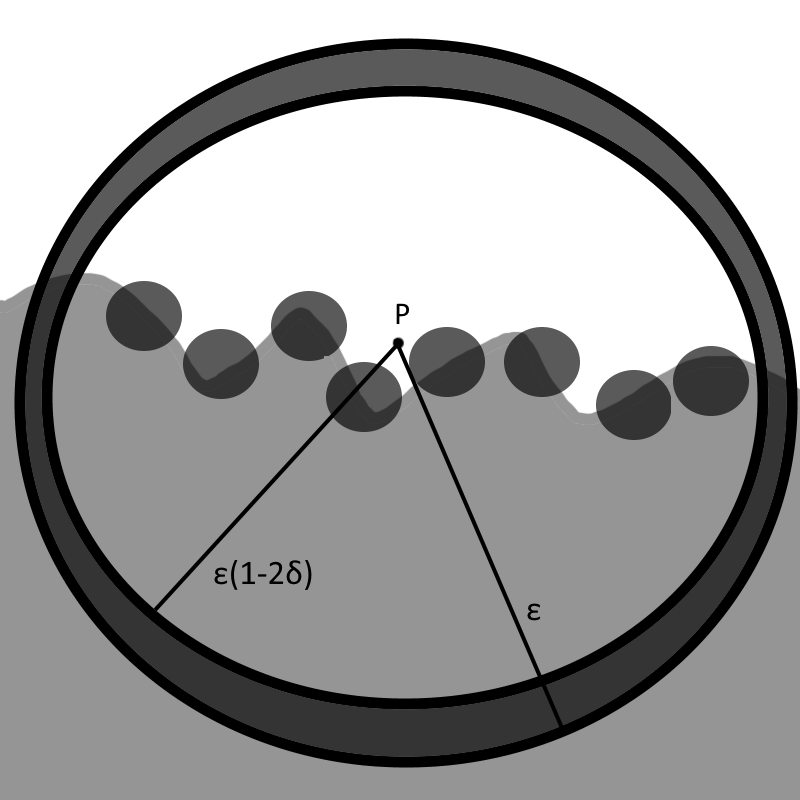
\includegraphics[width=0.4\textwidth]{covering lemma}
% \end{figure}

% \begin{sublemma}
% On $B_{1 - 2\sigma} \cap \{c\gamma^2 < \varphi < 1 - c\gamma^2\}$,
% $$(1_{V_0}(|\dif u| - Tu))_\varepsilon \lesssim_p \gamma |\dif u|_\varepsilon.$$
% \end{sublemma}
% \begin{proof}
% It follows from the definitions that for every $P \in B_\varepsilon$ and $Q \in V_0$, $\chi_\varepsilon(P - Q) \lesssim \varepsilon^{-d} \delta$,
% whence, by Proposition \ref{doubling dimension},
% \begin{align*}
% (1_{V_0}(|\dif u| - x\partial_zu))_\varepsilon &\lesssim \frac{\delta}{\varepsilon^d} \int_{B_\varepsilon} *|\dif u| \lesssim \frac{\delta}{\varepsilon}.
% \end{align*}
% Let $P \in B_\varepsilon$. Then by Lemma \ref{Giusti71}, there exists $c > 0$ such that if $\varphi \in (c\gamma^2, 1 - c\gamma^2)$, then there exists $Q \in \partial^* U$ such that $d(P, Q) < \varepsilon(1 - \gamma)$.
% If $d(Q, R) < \gamma\varepsilon/2$, then $d(P, R) < \varepsilon - \gamma\varepsilon/2$ and so $\chi_\varepsilon(P - R) \gtrsim \varepsilon^{-d}\gamma$ whenever $R \in B(Q, \gamma\varepsilon/2) =: W_0(P)$.
% We thus estimate
% $$\varepsilon^{-1} \gamma^{d - 1} \lesssim (1_{W_0(P)}|\dif u|)_\varepsilon \leq |\dif u|_\varepsilon$$
% and hence we obtain
% $$(1_{V_0}(|\dif u| - x\partial_zu))_\varepsilon(P) \lesssim \delta \gamma^{1 - d} |\dif u|_\varepsilon$$
% uniformly in $P$. Since $\delta = \gamma^d$, the claim holds.
% \end{proof}

The main result of this section is the following generalization of \cite[Lemma 7.5]{Giusti77}.
In the exposition of Giusti the statement is qualitative and only for $\Delta = 1$, but due to the lack of scale-invariance of $g$ it will be convenient for us to state the result in a quantitative matter and for $\Delta$ arbitrary.

\begin{proposition}[existence of mollification]\label{mollifier quant}
For every $0 < \varepsilon \lesssim 1$, there exists $\gamma_* > 0$ such that for every $0 < \Delta \lesssim 1$, every set $U$ of least perimeter in $B_\Delta$ such that
\begin{equation}\label{bootstrap the mollifier}
\gamma := \Delta^{1 - d} \int_{B_\Delta} \star |\dif 1_U| - T1_U < \gamma_*,
\end{equation}
and almost every $0 < t < 1$, there exists a set $V$ of $C^1$ perimeter in $B_{t\Delta}$, such that
\begin{align}
|V \cap B_{t\Delta}| &\leq \eta(V, t\Delta) + \varepsilon \gamma \Delta^{d - 1}, \label{mollifier quant1}\\
\left||U \cap B_{t\Delta}| - |V \cap B_{t\Delta}|\right| &\leq \varepsilon \gamma \Delta^{d - 1}, \label{mollifier quant2}\\
g^{-1}(\dif x^1, \normal_V) &\geq (1 - \varepsilon)\sqrt{\det g} \text{ on } B_{t\Delta(1 - \gamma^{O(1)})}, \label{mollifier quant4}
\end{align}
and for every $d-1$-form $\omega$ defined near $P$,
\begin{equation}
\left|\int_{B_{t\Delta}} \dif(1_U - 1_V) \wedge \omega\right| \leq \varepsilon \gamma \Delta^{d - 1} ||\omega||_{C^1}. \label{mollifier quant3}
\end{equation}
\end{proposition}
\begin{proof}
If the various assertions of this proposition fail, then there exist arbitrarily small $\varepsilon > 0$ such that we can find sets $(U_n)$ of least perimeter in $B_{\Delta_n}$ which are increasingly severe counterexamples in the sense that there exists a positive measure set of $t$ such that for every set $V$ of $C^1$ perimeter in $B_t$, at least one of (\ref{mollifier quant1}, \ref{mollifier quant2}, \ref{mollifier quant4}, \ref{mollifier quant3}) is false, in spite of the fact that for $\gamma_n$ defined by (\ref{bootstrap the mollifier}), one has $\gamma_n \to 0$.

After passing to a subsequence and applying the pigeonhole principle, we may assume that one of (\ref{mollifier quant1}, \ref{mollifier quant2}, \ref{mollifier quant4}, \ref{mollifier quant3}) fails on a positive measure set for every $n$, and moreover that $(\gamma_n) \in \ell^1$.
To obtain a contradiction we draw $t$ uniformly at random, let $w_n = (u_n)_{\Delta_n \gamma_n^4}$, let $c$ be as in Lemma \ref{main mollifier lemma}, and let $a_n = c\gamma_n^2$, $b_n = 1 - c\gamma_n^2$.
By the coarea formula, Proposition \ref{Coarea2},
$$\int_{B_{t\Delta_n}} \star |\dif w_n| = \int_0^1 |\partial^* \{w_n > y\} \cap B_{t\Delta_n}| \dif y \geq \int_{a_n}^{b_n} |\partial^* \{w_n > y\} \cap B_{t\Delta_n}| \dif y,$$
so by the mean value theorem, there exists $y_n \in (a_n, b_n)$ such that
\begin{equation}\label{MVT mollifier}
|\partial^* \{w_n > y_n\} \cap B_{t\Delta_n}| \leq \frac{1}{b_n - a_n} \int_{B_{t\Delta_n}} \star |\dif w_n|.
\end{equation}
We then set $V_n = \{w_n > y_n\}$, $v_n = 1_{V_n}$, so $V_n$ has $C^1$ boundary in $B_{t\Delta_n}$ by (\ref{claim 2 on main mollifier lemma}), and from (\ref{claim on main mollifier lemma}) and (\ref{T in coords}), on $B_{t\Delta_n - t\Delta_n \gamma_n^{1/(2(d - 1)}}$,
\begin{equation}\label{mollifier prop4}
g^{-1}(\dif x^1, \normal_{V_n}) = |\dif v_n|^{-1} g^{-1}(\dif x^1, \dif v_n) = |\dif v_n|^{-1} \sqrt{\det g} Tv_n \geq (1 - o(1)) \sqrt{\det g}.
\end{equation}
We moreover claim that almost surely,\begin{align}
|\partial V_n \cap B_{t\Delta_n}| &\leq \eta(V_n, \Delta_n) + o(\Delta_n^{d - 1} \gamma_n), \label{mollifier prop1}\\
\left|\int_{B_{t\Delta_n}} \star(|\dif u_n| - |\dif v_n|)\right| &\ll \Delta_n^{d - 1} \gamma_n, \label{mollifier prop2}
\end{align}
and for every $d-1$-form $\omega$ with $||\omega||_{C^1} \lesssim 1$,
\begin{equation}
\left|\int_{B_{t\Delta_n}} \dif (u_n - v_n) \wedge \omega\right| \ll \Delta_n^{d - 1} \gamma_n. \label{mollifier prop3}
\end{equation}
This claim contradicts the fact that at least one of (\ref{mollifier quant1}, \ref{mollifier quant2}, \ref{mollifier quant4}, \ref{mollifier quant3}) fails with positive probability for every $n$ and a fixed $\varepsilon$.

To establish the claim, we slightly modify the proof of \cite[Lemma 7.5]{Giusti77}.
By \cite[Lemma 7.2]{Giusti77}, Proposition \ref{doubling dimension}, and the fact that $\Delta_n \lesssim 1$,
$$\limsup_{n \to \infty} \Delta_n^{1 - d} \gamma_n^{-4} \int_{B_{t\Delta_n}} \star |u_n - w_n| \leq \limsup_{n \to \infty} \Delta_n^{-d} |\partial^* U_n \cap B_{t\Delta_n}| \lesssim 1$$
and hence almost surely,
$$||u_n - w_n||_{L^1(\partial B_{t\Delta_n})} \ll \Delta_n^{d - 1} \gamma_n^3.$$
So by \cite[Lemma 1.25]{Giusti77} and the fact that $y_n = c\gamma_n^2$,
\begin{equation}\label{trace of vn}
||u_n - v_n||_{L^1(\partial B_{t\Delta_n})} \lesssim \gamma_n^{-2} ||u_n - w_n||_{L^1(\partial B_{t\Delta_n})} \ll \Delta_n^{d - 1} \gamma_n.
\end{equation}
We moreover introduce 
$$f(s) = \sum_{n=1}^\infty \gamma_n \Delta_n^{1 - d} \int_{B_{s \Delta_n}} \star |\dif u_n|.$$
Then $f' \geq 0$, and by Proposition \ref{doubling dimension}, $f(1) \lesssim \sum_n \gamma_n < \infty$.
So almost surely,
$$f(t + \gamma_n^4) - f(t) \lesssim \gamma_n^4$$
and hence 
$$\int_{B_{(t + \gamma_n^4)\Delta_n} \setminus B_{t\Delta_n}} \star |\dif u_n| \lesssim \gamma_n \Delta_n^{d - 1}.$$
From \cite[Lemma 7.2]{Giusti77} and (\ref{MVT mollifier}) we conclude that almost surely,
\begin{equation}\label{difference of surface area}
|\partial V_n \cap B_{t\Delta_n}| \leq |\partial^* U_n \cap B_{t\Delta_n}| + o(\Delta_n^{d - 1} \gamma_n).
\end{equation}
Now (\ref{mollifier prop2}) follows from (\ref{trace of vn}), (\ref{difference of surface area}), and (\ref{a priori estimate 1}).
From (\ref{mollifier prop2}), (\ref{a priori estimate 1}) the fact that $U_n$ has least perimeter, and (\ref{trace of vn}), we also obtain (\ref{mollifier prop1}).
Finally we obtain (\ref{mollifier prop3}) by integration by parts: 
$$\left|\int_{B_{t\Delta_n}} \dif (u_n - v_n) \wedge \omega\right| \leq ||\omega||_{L^\infty} ||u_n - v_n||_{L^1(\partial B_{t\Delta_n})} + ||\dif \omega||_{L^\infty} \int_0^1 ||u_n - v_n||_{L^1(\partial B_{s\Delta_n})} \dif s.$$
The first term here is acceptable by (\ref{trace of vn}), and the second is also acceptable because (\ref{trace of vn}) holds with $t$ replaced with almost any $s$, so we can apply Fatou's lemma.
\end{proof}



%%%%%%%%%%%%%%%%%%%%%%%%%%%%%%%%%%%%%%%%%%%%%%%

\section{Plateau's equation}\label{DeGiorgiSection}
Having shown that we can reduce the study of sets of least perimeter to sets with $C^1$ and approximately least perimeter, our next task is to represent such sets as graphs of approximate solutions to a Plateau-type equation.

\subsection{Derivation}
Let $(x^\mu)$ and $\psi$ be as above. We introduce the projection
\begin{align*}
    \Pi: M &\to \Omega \subseteq \RR^{d - 1}\\
    x &\mapsto (x^1, \dots, x^{d - 1}).
\end{align*}
If $\omega$ is a $C^r$ function $\Omega \to \RR$, we introduce the locally closed $C^r$ embedding
\begin{align*}
    \Psi_\omega: \Omega &\to M \\
    x &\mapsto (\omega(x), x^1, x^2, \dots, x^{d - 1})
\end{align*}
which identifies $\Omega$ with the ``graph'' $N_\omega$ of $\omega$, which is a hypersurface in $M$.

For the construction of the Plateau equation we shall need the following definitions from exterior linear algebra.

\begin{definition}
Let $v_1, \dots, v_{d - 1} \in T_QM$.
The \dfn{Gram form} of $v_1, \dots, v_{d - 1}$ is the quadratic form on $\spn(\partial_1, \dots, \partial_{d - 1})$ defined by
$$\Gram(v_1, \dots, v_{d - 1})_{ij} = g(v_i, v_j).$$
The \dfn{cross product} $v_1 \times \cdots \times v_{d - 1}$ of vectors $v_1, \dots, v_{d - 1} \in T_QM$ is defined to be the vector $v_0$
such that:
\begin{enumerate}
\item $g(v_0, v_i) = 0$,
\item $((-1)^{d - 1} v_0, v_1, \dots, v_{d - 1})$ is positively oriented, and
\item $g(v_0, v_0) = |\det \Gram(v_1, \dots, v_{d - 1})|$.
\end{enumerate}
\end{definition}

\begin{proposition}[construction of Plateau energy]\label{construction of Plateau energy}
There exists a family of Riemannian metrics $\slashed g^{(y)}$ on $\Omega$ such that
\begin{equation}\label{decay of slashed metric}
\slashed g^{(y)}_{ij} = \delta_{ij} + O(|x|^2 + y^2)
\end{equation}
and for every $\omega \in C^r(\Omega)$, $r \geq 1$, the \dfn{Plateau energy}
\begin{equation}\label{Plateau energy}
\Lagrange[\omega, \grad_{\slashed g^{(\omega)}} \omega] := e^{O(|x|^2)} \sqrt{1 + |\grad_{\slashed g^{(\omega(x))}} \omega(x)|^2_{\slashed g^{(\omega(x))}(x)}} \dif x^1 \wedge \cdots \dif x^{d - 1}
\end{equation}
is the pullback by $\Psi_\omega$ of the area form on $N_\omega$.
Moreover, the conormal $1$-form to $N_\omega$ is
\begin{equation}\label{conormal}
\normal_\mu(x, \omega(x)) = \frac{e^{O(|x|^2)}}{\sqrt{1 + |\grad_{\slashed g^{(\omega(x))}} \omega(x)|_{\slashed g^{(\omega(x))}(x)}^2}} (\delta^0_\mu - \delta^i_\mu \partial_i \omega(x)).
\end{equation}
Finally, if $g$ is analytic then so is $\slashed g$.
\end{proposition}
\begin{proof}
TODO
\end{proof}

We shall call the Euler-Lagrange equation for $\Lagrange$ the \dfn{Plateau equation} with respect to $\slashed g$.
Since $\Lagrange$ is a perturbation of the euclidean Plateau energy $\sqrt{1 + |\grad \omega|^2}$, the Plateau equation is a nonlinear variational elliptic PDE of second order and smooth coefficients on $\RR^{d - 1}$.
In particular, $C^1$ weak solutions of the Plateau equation are smooth, and even is analytic if $\slashed g$ is analytic (see \cite[\S8.3.2]{evans2010partial} and the references therein), ergo:

\begin{corollary}\label{C1 implies smooth}
Let $N$ be a $C^1$ minimal hypersurface in $M$. Then $N$ is smooth, and if $g$ is analytic, then $N$ is analytic.
\end{corollary}

\subsection{A multiplicative gain}
We now apply the strategy of Miranda \cite[Teorema 4.3]{Miranda66} to obtain a multiplicative gain on the mean oscillation of the Plateau energy $\Lagrange[\omega, \grad_{\slashed g} \omega]$ when one passes from a dyadic scale $r$ to its child $r/2$.
To motivate why the same argument should work in our context, we note that the result of Miranda is effective when $|\grad \omega| \ll 1$.
So we shall linearize the Plateau equation about the constant solution $\omega = \omega(0)$.
From the expansion (\ref{decay of slashed metric}), we can then replace $\slashed g^{(y)}$ with the euclidean metric. Taylor expanding (\ref{Plateau energy}) to second order in $\grad \omega$ and approximating $e^{O(|x|^2)}$ by $1$, we arrive at the \dfn{Dirichlet energy}
$$\DirL[\grad \omega] := \frac{1}{2} |\grad \omega|^2,$$
whose Euler-Lagrange equation is the euclidean Laplace equation, just as in the argument of Miranda.

\printbibliography

\end{document}
